\documentclass[oneside, 11pt]{article}

\usepackage[T1]{fontenc}
\usepackage[utf8]{inputenc}
\usepackage[english]{babel}

\usepackage{fouriernc}
\usepackage[detect-all, binary-units, separate-uncertainty=true,
            per-mode=symbol, retain-explicit-plus, retain-unity-mantissa=false]{siunitx}

\usepackage{setspace}
\setstretch{1.2}

\setlength{\parskip}{\smallskipamount}
\setlength{\parindent}{0pt}

\usepackage[headheight=14pt]{geometry}
\geometry{marginparwidth=0.5cm, verbose, a4paper, tmargin=3cm, bmargin=3cm,
          lmargin=2cm, rmargin=2cm}

\usepackage{float}

\usepackage[fleqn]{amsmath}
\numberwithin{equation}{section}
\numberwithin{figure}{section}

\usepackage{graphicx}
\graphicspath{{images/}{../../../images/}}

\usepackage{tikz}
\usetikzlibrary{shapes}
\usetikzlibrary{plotmarks}

\newcounter{Exercise}
\setcounter{Exercise}{1}
\usepackage{xcolor}
\definecolor{shadecolor}{gray}{0.9}
\usepackage{framed}
\usepackage{caption}

\usepackage{url}


\usepackage{fancyhdr}
\pagestyle{fancy}
\fancyhf{}
\rhead{\thepage}
\renewcommand{\footrulewidth}{0pt}
\renewcommand{\headrulewidth}{0pt}

\fancypagestyle{firststyle}
{
    \fancyhf{}
    \rhead{\thepage}
    \cfoot{
\includegraphics[height=30pt]{HiSPARClogo}}
    \rfoot{
\includegraphics[height=25pt]{CCbysa}}
    \lfoot{
\includegraphics[height=30pt]{NIKHEFlogo}}
    \renewcommand{\footskip}{50pt}
    \renewcommand{\footrulewidth}{0.1pt}
    \renewcommand{\headrulewidth}{0pt}
}

\newcommand{\figref}[1]{Figuur~\ref{#1}}

\newcommand{\hisparc}{\textsmaller{HiSPARC}\xspace}
\newcommand{\kascade}{\textsmaller{KASCADE}\xspace}
\newcommand{\sapphire}{\textsmaller{SAPPHiRE}\xspace}
\newcommand{\jsparc}{\textsmaller{jSparc}\xspace}
\newcommand{\hdf}{\textsmaller{HDF5}\xspace}
\newcommand{\aires}{\textsmaller{AIRES}\xspace}
\newcommand{\csv}{\textsmaller{CSV}\xspace}
\newcommand{\python}{\textsmaller{PYTHON}\xspace}
\newcommand{\corsika}{\textsmaller{CORSIKA}\xspace}
\newcommand{\labview}{\textsmaller{LabVIEW}\xspace}
\newcommand{\daq}{\textsmaller{DAQ}\xspace}
\newcommand{\adc}{\textsmaller{ADC}\xspace}
\newcommand{\hi}{\textsc{h i}\xspace}
\newcommand{\hii}{\textsc{h ii}\xspace}
\newcommand{\mip}{\textsmaller{MIP}\xspace}
\newcommand{\hisparcii}{\textsmaller{HiSPARC II}\xspace}
\newcommand{\hisparciii}{\textsmaller{HiSPARC III}\xspace}

\DeclareSIUnit{\electronvolt}{\ensuremath{\mathrm{e\!\!\:V}}}

\DeclareSIUnit{\unitsigma}{\ensuremath{\sigma}}
\DeclareSIUnit{\mip}{\textsmaller{MIP}}
\DeclareSIUnit{\adc}{\textsmaller{ADC}}

\DeclareSIUnit{\gauss}{G}
\DeclareSIUnit{\parsec}{pc}
\DeclareSIUnit{\year}{yr}




%document details
\author{N.G. Schultheiss \\ translated and adapted by K. Schadenberg}
\date{}
\title{Grinding Lenses}


\begin{document}
\maketitle

\section{Introduction}
This module `Grinding Lenses follows the module `Lenses' or `Parabolic Mirrors' and can lead to `Telescopes'. When you completed all these modules you should be able to make your own telescope with the help of the module `Making your own telescope' and explain how it works. This module, like `Parabolic Mirrors' is more technical then the previous ones because it focusses more on constructing a lens then on the mathematics behind the workings of a lens.

It is assumed that you know and understand the Pythagorean theorem.

\section{Constructing spheres}
A sphere is a three-dimensional surface, all points of which are equidistant from a fixed point; the centre. This distance is called the radius $r$. Using the Pythagorean theorem we can describe the surface of a sphere (in Cartesian coordinates) in a single mathematical formula:
\begin{equation}
x^2 + y^2 + z^2 = r^2 \label{eq:sphere}
\end{equation}

Lets see what happens when we cut away a slice of the sphere. We take a sphere with a radius of 5.0~cm and take away a 1.0~cm thick slice. We made the cut at $z=4.0$~cm.
\begin{equation*}
x^2 + y^2 + 4.0^2 = 5.0^2 ~~\Rightarrow~~ x^2 + y^2 = 3.0^2
\end{equation*}
This equation tells us that the cut made is circular in shape and has a radius of 3.0~cm. Making a plano convex lens is therefore easy, just slice of a piece of a glass sphere. First however we need to obtain a (part of a) glass sphere.

Grinding lenses can be done by rotating a glass pane and `cutting' away glass from the top with a rotating cylinder which is placed at an angle to the rotating plane. Machining in this fashion will result in a partial sphere. A suitable cylinder to use if you want to try this process for yourself is a hole saw. See figure \ref{fig:grinding_setup} for a possible setup to grind lenses.

\begin{figure}\begin{center}
\begin{picture}(0,0)%
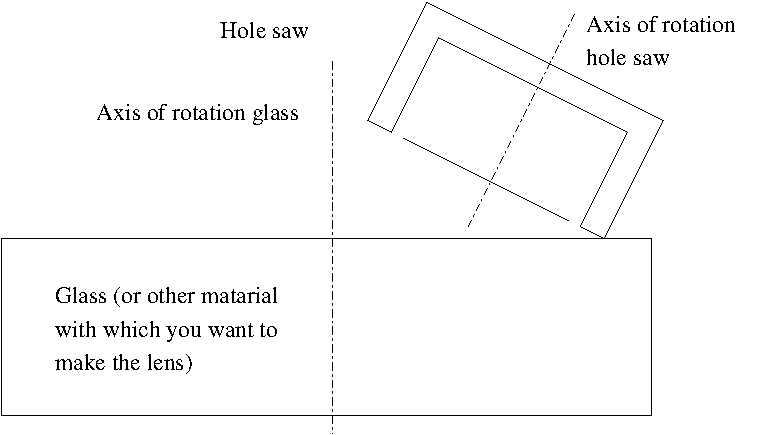
\includegraphics{grinding_setup}%
\end{picture}%
\setlength{\unitlength}{4144sp}%
%
\begingroup\makeatletter\ifx\SetFigFont\undefined%
\gdef\SetFigFont#1#2#3#4#5{%
  \reset@font\fontsize{#1}{#2pt}%
  \fontfamily{#3}\fontseries{#4}\fontshape{#5}%
  \selectfont}%
\fi\endgroup%
\begin{picture}(5835,3309)(-11,-2728)
\end{picture}%
\caption{A setup to grind lenses.}\label{fig:grinding_setup}
\end{center}\end{figure}

It is important to align the axis of rotation in such a way that axis of the hole saw cuts crosses the axis of the rotating pane. Trying this process with glass can be quite dangerous, a safer alternative is Plexiglas (Poly(methyl methacrylate), PMMA). If everything is rotating properly we end up with a nice sphere (without a strange tip at the top). The hole saw however cuts away material quite crude, we therefore do not obtain a nice smooth surface.

After cutting we can sand down the surface to make it smoother. To do this take a piece of tubing with the same diameter as the hole saw  and cover the end with sandpaper. Use this `sander' in the same way as the hole saw. A different method uses grinding paste made from water and fine sand to polish the surface. Multiple polishing steps are needed, each with a finer polishing paste. Scouring cleaning agents can be used as an intermediate coarseness and copper polish as the finest polish. When we are done with polishing we end up with a plano convex lens. The lens makers equation can be used to calculate its strength.

\end{document}
